%   Filename    : chapter_4.tex 
\chapter{Research Methodology}

In this study, we will conduct the steps outlined in each of the following sections.

\section{Data Gathering}

In data gathering, we will source Filipino news articles, both fake and authentic, from the internet.

Specifically, we will follow the data-gathering methodology outlined in the work of \cite{cruz2020localization} to refrain from reinventing the wheel and to ensure consistency between fresh and old data. To augment the Fake News Filipino dataset from their study with a dataset of our own, we will source fake news articles via web scraping from various fraudulent websites tagged by Verafiles. Authentic news will be sourced from trusted mainstream providers such as The Philippine Star and ABS-CBN. The text will be encoded in UTF-8. Minimal preprocessing of the text will be done to preserve features such as misspelled words and incorrect punctuation. The news articles will be mostly Filipino with a few words in the English vernacular. Scraped fake news and authentic news will be labeled accordingly as Fake or Real.

\section{Model Training and Data Processing}
\label{sec:ModelTraining}

Figure \ref{fig:Model} shows the steps in model training and data processing. Generally, we will tokenize the text input, extract the features, train the models using the extracted features, and classify the input text using ensemble learning.

Specifically, we will tokenize the text using a pre-trained BPE tokenizer. Linguistic features highlighted by \citeA{fernandez-2019} as well as \citeA{fayaz-2022} will be used in training our models. Table \ref{tab::Features} describes the features to be extracted and specifies their predictors. These features include traditional or surface-based  features such as word count, sentence count, and character count. We will extract these features via a library of Python scripts designed specifically for the extraction of Filipino linguistic features \cite{imperial-2020, imperial-2021}. Through the same library, we will also extract syllabic features based on the prescribed Philippine orthography, lexical features such as type-token ratio, morphological features such as morphemes, and language model features such as perplexity. Additionally, the frequency of misspelled words, which has not been investigated as a linguistic feature of Filipino texts in previous studies, will be appended to the feature space. We will vectorize the tokens with TF-IDF, extracting unigrams, bigrams, and trigrams as well as bag-of-words. We will train the following classifiers on the extracted features: Multinomial Naive Bayes, Logistic Regression, Random Forest, Support Vector Classifier (SVC), and various Voting Classifiers.

\begin{figure}[h]
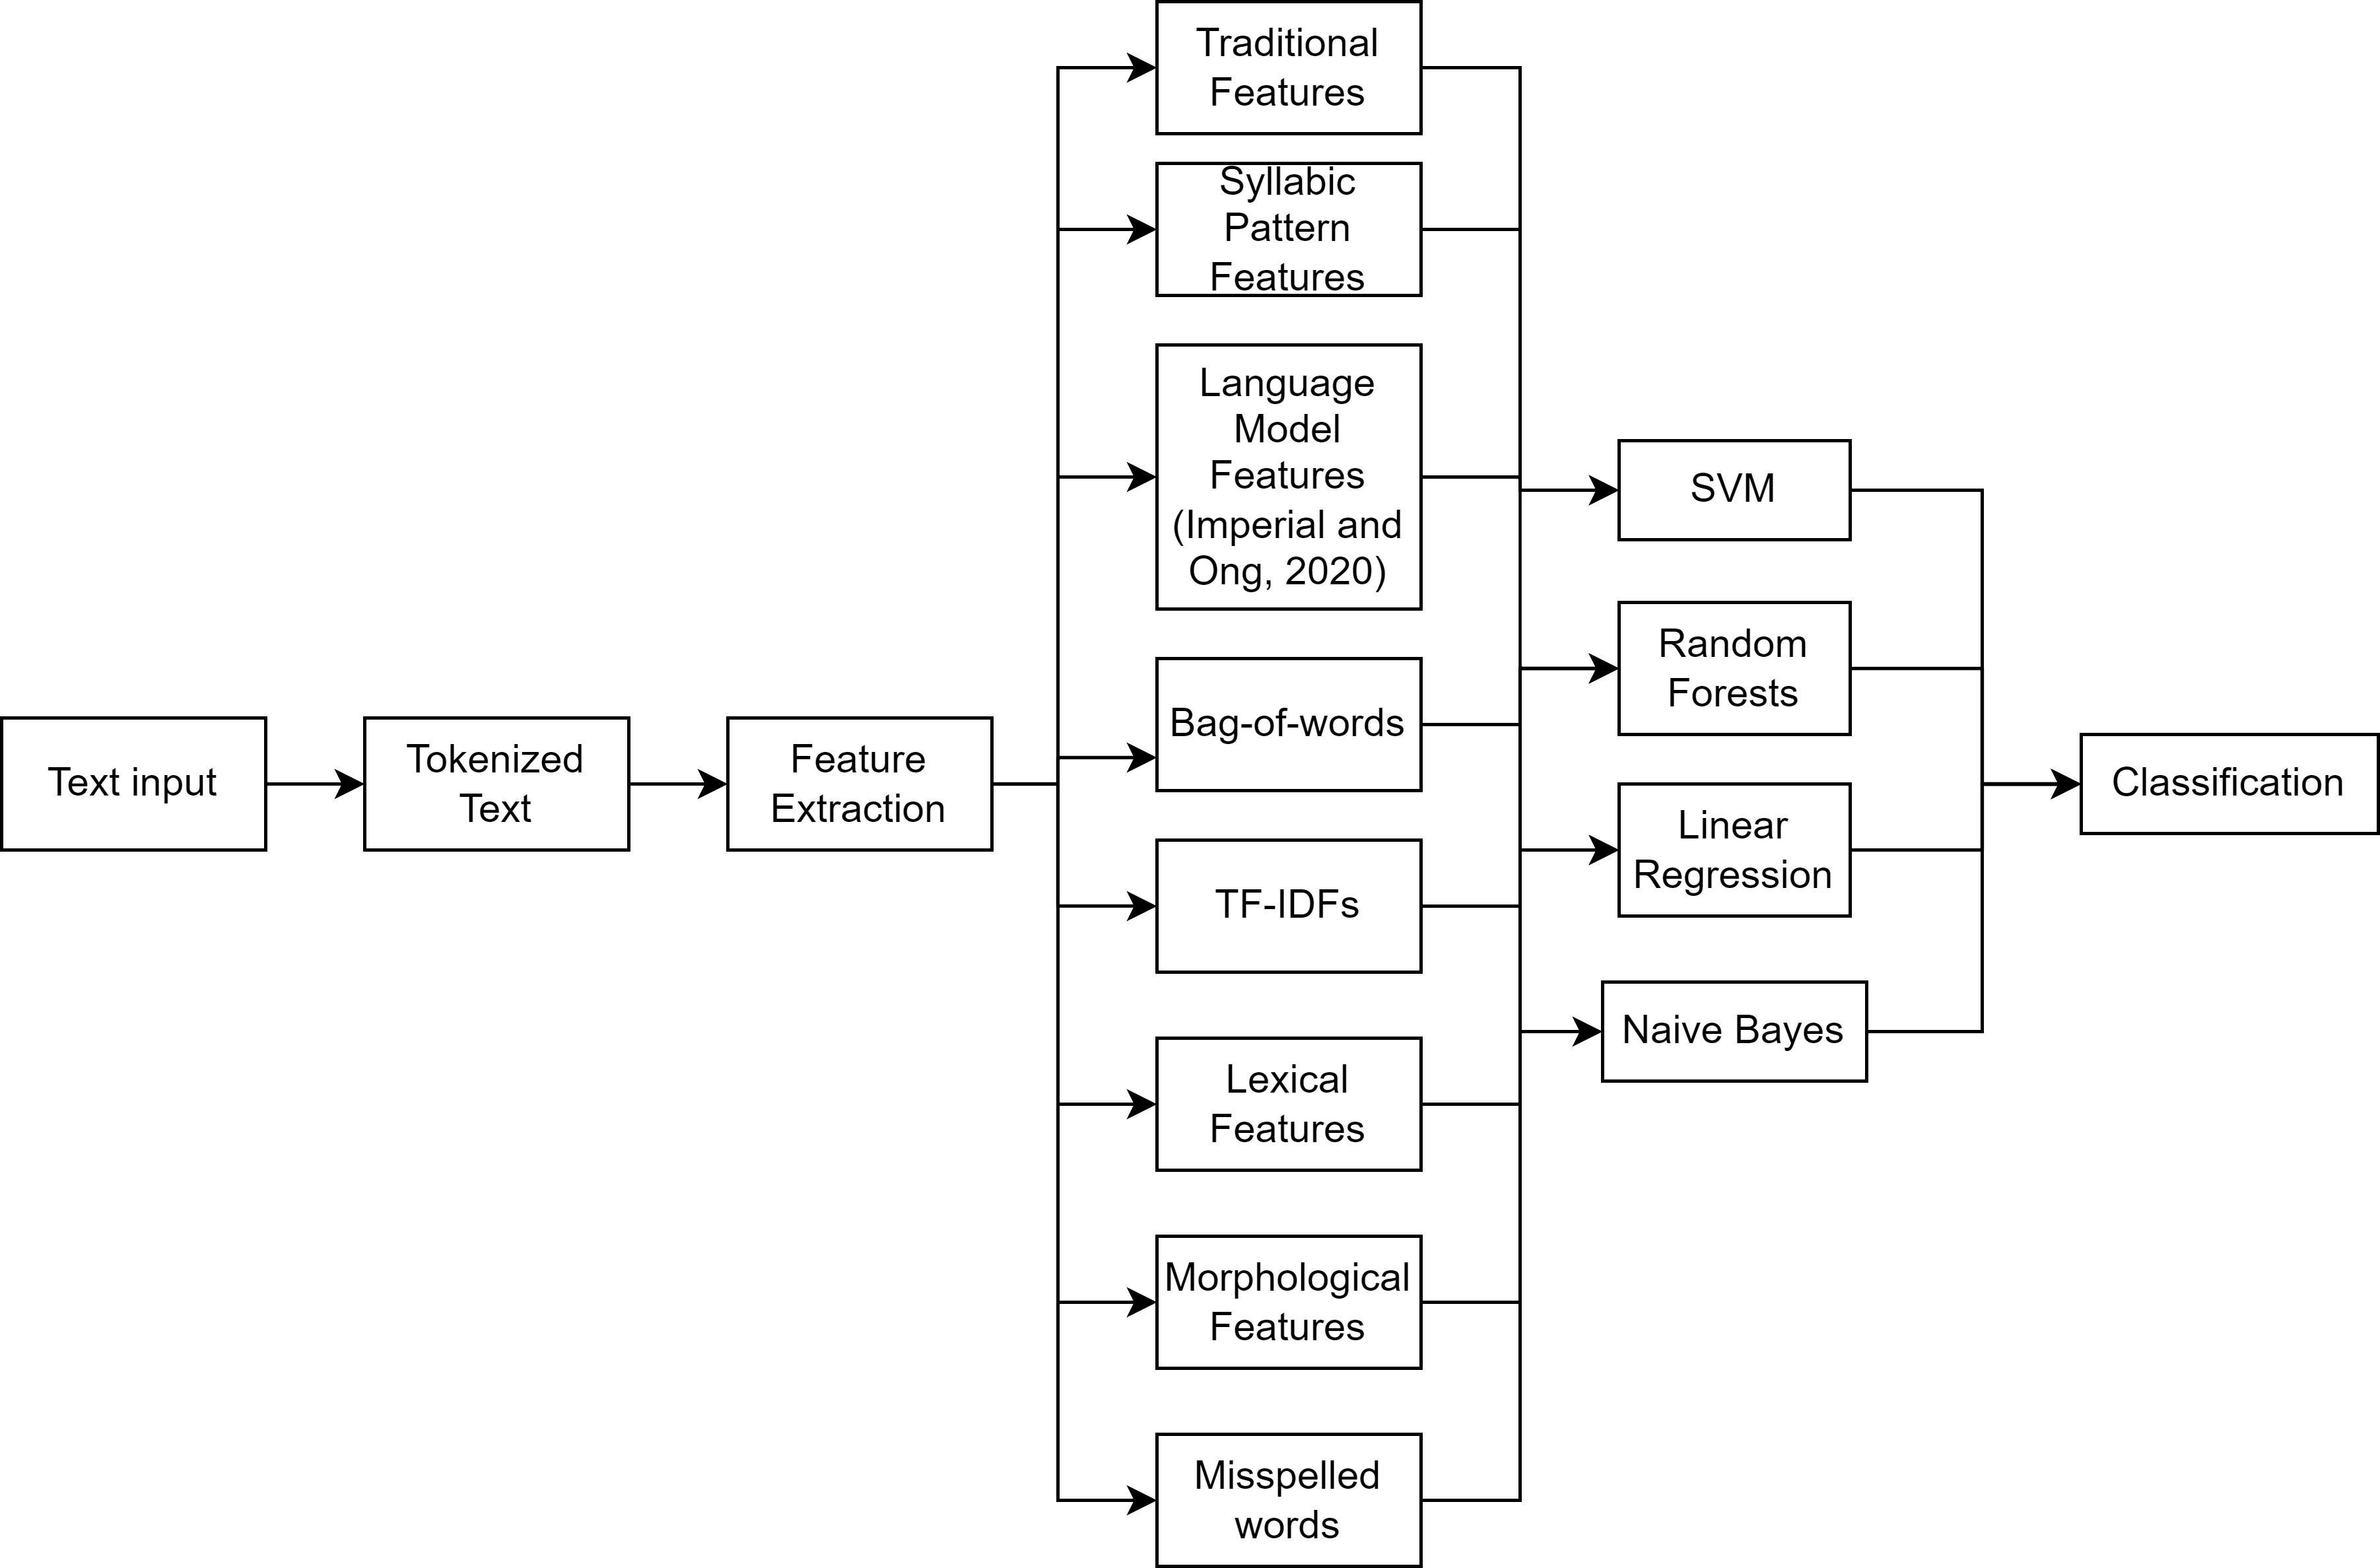
\includegraphics[width=\textwidth,height=\textheight,keepaspectratio]{figures/Model Training.png}
  \caption{Data Processing and Model Training}
  \label{fig:Model}
\end{figure}

\clearpage

\begin{tabularx}{\textwidth}{|X|X|X|}
     \hline Feature  & Description & Predictors \\ \hline
     \endfirsthead

     \hline
     \multicolumn{3}{|r|}
     {Continued from previous page.} \\
     \hline
     Feature  & Description & Predictors \\ \hline
     \endhead

     \hline \multicolumn{3}{|r|}{{Continued on next page...}} \\ \hline
     \endfoot
     
     \hline
     \caption{Descriptions and predictors of features.}
     \endlastfoot

     Bag-of-words & Unordered collection of words. & Bag-of-words model of the input text. \\
     \hline
     TF-IDF & Word to document ratio in the corpus. & TF-IDF using n-gram values of \{ 1, 2, 3\} \\
     \hline
     Misspelled words & Misspelled words in the input text. & Total misspelled word count. \\
     \hline
     Traditional & Traditional or Surface-based features based on counts and frequencies & Total word, sentence, phrase, polysyllabic word counts. Average word length, sentence length, syllable per word. \\
     \hline
     Syllabic Pattern & Syllable pattern densities based on the prescribed Philippine orthography & Prescribed Philippine orthography \{v, cv, vc, cvc, vcc, cvcc, ccvc, ccvcc, ccvccc\}, where c and v are consonant and vowel notations. \\
    \hline
    Lexical & Lexical or context carrying features using part-of-speech categories. & Type-token variations (regular, logarithmic, corrected, root). Noun and verb token ratio. Lexical density. Foreign word and compound word density.\\
    \hline
    Morphological & Morphological features based on verb inflection. & Densities of  foci of verbs based on tense: \{actor, object, benefactive, locative, instrumental, referential\}. Densities of various foci of verbs based on aspect: \{infinitive, perfective, imperfective, contemplative, participle, recent-past, auxiliary\}.\\
    \hline
    Language Model &  Language model features based on perplexity used by \citeA{imperial-2020} & Language models trained on three levels of the external DepEd Commons corpus using n-gram values of \{1, 2, 3\}.
\label{tab::Features}
\end{tabularx}


% %%
% \begin{table}[h]
%     \centering
%     \begin{tabularx}{\textwidth}{|X|X|X|}
%          \hline
%          Feature  & Description & Predictors \\
%          \hline
%          Bag-of-words & Unordered collection of words. & Bag-of-words model of the input text. \\
%          \hline
%          TF-IDF & Word to document ratio in the corpus. & TF-IDF using n-gram values of \{ 1, 2, 3\} \\
%          \hline
%          Misspelled words & Misspelled words in the input text. & Number of misspelled words \\
%          \hline
%          Traditional & Traditional or Surface-based features based on counts and frequencies & Total word, sentence, phrase, polysyllabic word counts. Average word length, sentence length, syllable per word. \\
%          \hline
%          Syllabic Pattern & Syllable pattern densities based on the prescribed Philippine orthography & Prescribed Philippine orthography \{v, cv, vc, cvc, vcc, cvcc, ccvc, ccvcc, ccvccc\}, where c and v are consonant and vowel notations. \\
%         \hline
%         Lexical & Lexical or context carrying features using part-of-speech categories. & Type-token variations (regular, logarithmic, corrected, root). Noun and verb token ratio. Lexical density. Foreign word and compound word density.\\
%         \hline
%         Morphological & Morphological features based on verb inflection. & Densities of various foci of verbs based on tense: \{actor, object, benefactive, locative, instrumental, referential\}. Densities of various foci of verbs based on aspect: \{infinitive, perfective, imperfective, contemplative, participle, recent-past, auxiliary\}.\\
%         \hline
%         Language Model &  Language model features based on perplexity used by \citeA{imperial-2020} & Language models trained on three levels of the external DepEd Commons corpus using n-gram values of \{1, 2, 3\}.\\
%         \hline
%     \end{tabularx}
%     \caption{Table of features}
%     \label{tab:my_label}
% \end{table}
% %%

\section{System Deployment}

\subsection{System Architecture}

Our system will consist of three components: a machine learning model deployed as a microservice, an application programming interface (API) running via a cloud server infrastructure to host the model, and a cross-browser extension to interface with the API.

We will utilize a cloud server infrastructure through Render (a platform as a service). We have chosen Render because its free tier presents numerous advantages such as automated load balancing, a generous bandwidth and build time allocation, and integration with GitHub — changes can be deployed within a few seconds of pushing to a pipelined repository \cite{render-docs}. While it is not suitable for enterprise-scale production, it is suitable for rapid prototyping and deployment of full-stack web applications.

For our client, we will utilize a browser extension deployed via Tampermonkey, a cross-browser extension manager. Tampermonkey allows users to enhance the functionality of web pages via injecting a script (written in JavaScript) into the page. We have chosen Tampermonkey as it is one of the most popular browser extensions available on mainstream web browsers (e.g. Google Chrome, Mozilla Firefox, Microsoft Edge, Safari, Opera, Next), it grants web developers the ability to write browser-independent code, and it provides a library of extensions to make them easy to deploy and install \cite{tampermonkey-website}.

Python is our go-to in the backend as it is the programming language of choice when it comes to machine learning; we provide ease of compatibility between our API and our microservice. We will deploy both our model and our API via FastAPI, a modern web framework for building RESTful APIs in Python. We have chosen FastAPI because it boasts very high performance (one of the fastest Python web frameworks available, on par with NodeJS and Go), it is easy to use and has a smooth learning curve, and it complies with open standards for API (OpenAPI and JSON Schema) \cite{fastapi-website}.

\subsection{System Usage}

As Figure \ref{SystemFlowchart} shows, the user interacts with the FaKe browser extension while reading a Filipino language news article. A stable internet connection is required to establish communication between the FaKe browser extension and API.

The FaKe browser extension scrapes the paragraph body of the article and packs it in a JSON. This packed JSON is sent to the API that hosts the machine learning model. The API unpacks the JSON and extracts Filipino lingustic features from the article text. The API employs exactly the same modules used in the extraction of Filipino linguistic features during model training. No sensitive information such as user credentials or IP addresses is transmitted. Once the Filipino linguistic features are extracted, the API uses the model microservice to make predictions on these features. The model identifies whether the article is fake or not, entailing a waiting period of up to 30 seconds. The waiting period hinges on the state of the server and the length of the article. If an error during this exchange occurs, the user is notified and prompted to try again. However, if no error occurs and the model successfully predicts whether the article is fake or not, the API returns the prediction as a response JSON to the browser extension. The browser extension unpacks this response JSON and displays the prediction (fake or real) to the user.

\begin{figure}[h]
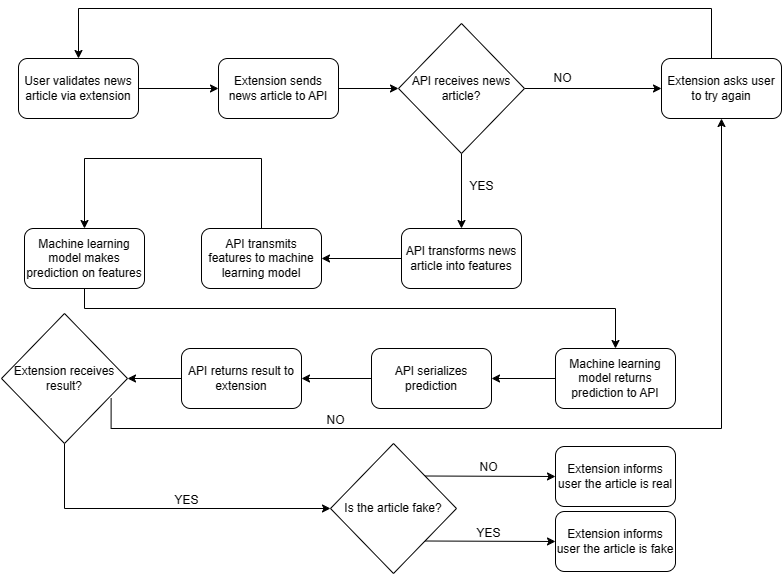
\includegraphics[width=\textwidth,height=\textheight,keepaspectratio]{figures/FakeSystemFlowchart.png}
  \caption{FaKe High Level System Flowchart}
  \label{SystemFlowchart}
\end{figure}
\clearpage

\subsection{System Limitations}

As of the time of writing, the FaKe API is being hosted on a cloud server that spins down after long periods of inactivity. Free deployment instances at Render spin down after 15 minutes of no inbound traffic \cite{render-docs}, requiring time to spin back up. This means that it takes longer to respond to requests if no request has been sent for a long time. Once the server is active, requests may be promptly handled.

The FaKe browser extension as a tool only functions reliably on news articles written in the Filipino language. Results from making predictions on news articles in English or other languages are unreliable at best. However, the FaKe browser extension has no way of limiting its usage to Filipino language news articles. Furthermore, predictions made by the FaKe browser extension may be inaccurate and may not reflect real-world events. Thus, the responsible usage of the FaKe browser extension rests with the user. In this regard, we advocate for the hybrid approach in detecting fake news, wherein the employment of the FaKe browser extension is accompanied by dutiful and informed fact-checking. We make no claims that FaKe is a singular catch-all solution to detecting Filipino language fake news.

\section{Calendar of Activities}

Table \ref{tab:timetableactivities} shows a Gantt chart of the activities to be conducted in this study.  Each bullet represents approximately one week worth of activity.

%
%  the following commands will be used for filling up the bullets in the Gantt chart
%
\newcommand{\weekone}{\textbullet}
\newcommand{\weektwo}{\textbullet \textbullet}
\newcommand{\weekthree}{\textbullet \textbullet \textbullet}
\newcommand{\weekfour}{\textbullet \textbullet \textbullet \textbullet}

%
%  alternative to bullet is a star 
%
\begin{comment}
   \newcommand{\weekone}{$\star$}
   \newcommand{\weektwo}{$\star \star$}
   \newcommand{\weekthree}{$\star \star \star$}
   \newcommand{\weekfour}{$\star \star \star \star$ }
\end{comment}



\begin{table}[ht]   %t means place on top, replace with b if you want to place at the bottom
\centering
\caption{Timetable of Activities} \vspace{0.25em}
\begin{tabular}{|p{2in}|c|c|c|c|c|c|c|} \hline
\centering Activities (2023) & Jan & Feb & Mar & Apr & May\\ \hline
Finalize Model and Features      & ~~~\weekone & \weekfour &  &  & \\ \hline
Finalize System Implementation      & ~~~\weekone & \weekfour &  &  & \\ \hline
Model Training and Testing     &   &  & ~\weekthree~~~ &  & \\ \hline
Model Implementation     &   &  & ~~~~\weekone & \weektwo~~~ &  \\ \hline
Documentation & ~~~\weekone & \weekfour & \weekfour & \weekfour & \weekfour \\ \hline
\end{tabular}
\label{tab:timetableactivities}
\end{table}

